\subsection{\acrshort{lc/ms} Analysis of Whole Grain Barley}
The elution patterns of barley flour chromatograms (shown in Appendix) were mostly similar. Elution time of several peaks slightly deviated, but all within 0.02 min.

However, one major difference of the chromatograms was, bran powder had higher intensities than endosperm powders for some peaks. For example, in negative mode, bran powder had double intensities for peaks with retention time (min) 3.84, 3.97, 4.43 compared with endosperm powder.
The large difference could be explained by bran powder containing more 'whole grain' part. The compound in this part was more soluble in ethanol. But errors originated from the extraction was also possible.

\subsection{Data-preprocess}
After data-preprocessing, 1719 features were detected in positive mode; in negative mode, 3304 features were detected. 
Based on previous experience, it was very common to observe that more features were detected in negative mode than positive mode.

It could be explained by, either the instrument performs better in negative mode having a higher resolving power, or, some metabolites could be ionized easier in negative mode than positive mode, e.g. glucuronate conjugates.

\subsection{\acrshort{pca} Modeling}
%PCA
\acrshort{pca} modeling results were shown in Figure \ref{fig:pca}. In score plot, \acrfull{aw} and \acrfull{ab} can not be well separated. 

\acrshort{pca} can also detect outliers and be used for data quality control\cite{Scalbert2014}. 
In both modes, pooled samples located tightly near the center, which indicated that the data had a high quality. 
Two subjects were detected as outliers (outside 95\% confidence level limit) in both modes. 
We investigated raw data and observed that these two subjects almost showed high intensities in all variables. 
The reason could be their urine samples were too concentrated.

This is why metabolomics research could be very complex.
Although subjects were treated with the same intervention and biofluids were collected, processed and analyzed in the same way. But the metabolome could vary a lot between individuals.
Unlike laboratory animals, humans are free-living individuals. Metabolome could be affected by a lot of external factors, such as genes, living environments and health statues.

In this case, concentrated urine could be simply attributed to that these individuals did not drink enough water. These two subjects were not removed in further study.
\begin{figure}[h]
    \centering
    \includegraphics[scale=0.43]{images/pca_score.png}
    \caption{PCA score plot (AW= After Wheat, AB= After Barley, POOL= pooled samples)}
    \label{fig:pca}
\end{figure}

\subsection{\acrshort{plsda} Modeling and Variable Selections}
%PLSDA
\acrshort{plsda} modeling selected 72 variables out of 1719 features in positive mode; 86 variables out of 3304 features in negative mode.  These selected variables had high \acrshort{vip} value and selectivity ratio.

Although they can differentiate barley and wheat intake, not all of them were classified as potential biomarkers for barley intake. 
\begin{figure}[h]
    \centering
    \includegraphics[scale=0.36]{images/marker1.png}
    \caption{Variables Selected by PLSDA modeling but not classified as potential barley intake biomarkers (AW= After Wheat, AB= After Barley, POOL= pooled samples)}
    \label{fig:marker1}
\end{figure}
\begin{figure}[H]
    \centering
    \includegraphics[scale=0.36]{images/barley_marker.png}
    \caption{Intensity differences of potential barley intake biomarkers in different intervention time-points (AW= After Wheat, AB= After Barley, POOL= pooled samples)}
    \label{fig:selected}
\end{figure}
\clearpage
For example, as shown in Figure \ref{fig:marker1} (left), the intensity of this variable got suppressed after barley intake. This could be an endogenous metabolite suppressed by barley intake. In Figure \ref{fig:marker1} (right), this variable could be a potential biomarker for whole grain wheat intake. Because it had lower value in \acrshort{ab}, \acrshort{bb}, \acrshort{bw} but increased intensities after whole grain wheat intake.

%Potential biomarkers selection
Potential biomarkers for barley intake were further selected based on the criterials as described before to perform \acrshort{ms/ms} analysis for identification. Within these potential biomarkers, 5 were from negative mode and 1 was from positive mode. Figure \ref{fig:selected} showed intensities of biomarkers (part) in different time-points before and after intervention.

\subsection{\acrfull{ms/ms} and Identification of Potential Biomarkers}
\subsubsection{m/z 231.0870}
This ion was detected in negative mode. Intensity of this ion was too low to be detected in \acrshort{ms/ms}. Moreover, there was no feasible hints in the database. Possible formulas were summarized in Figure \ref{fig:231p0870}.
\begin{figure}[h]
    \centering
    \includegraphics[scale=0.5]{images/231p0870.pdf}
    \caption{Possible formulas of ion m/z 231.0870}
    \label{fig:231p0870}
\end{figure}

\subsubsection{m/z 775.3401}
This ion was detected in negative mode. It was annotated as the dimer of [C\textsubscript{18}H\textsubscript{28}O\textsubscript{9}-H]\textsuperscript{-} with neutral mass 388.1735. However, the intensities of both monomer and dimer were too low to be detected in \acrshort{ms/ms}. No feasible hints existed in the database.

\subsubsection{m/z 216.9995 - phenol or polyphenol metabolite}
This ion was detected in negative mode. 
\begin{figure}[h!]
    \centering
    \includegraphics[scale=0.46]{images/216d9995.pdf}
    \caption{Possible structures of ion m/z 216.9995}
    \label{fig:216p9995}
\end{figure}
Although this potential biomarker can distinguish barley and wheat intake, the intensity of this ion was too low to be detected in \acrshort{ms/ms}. In addition, this ion was not detected in barley samples. The reason could be either it was not ionized or it was bio-transferred. 

From HMDB database\cite{hmdb}, several feasible compounds matched its mass. Figure \ref{fig:216p9995} summarized the feasible structures. These compounds were all either detected or predicted metabolites of polyphenols, phenols and bezoic acids.

4-hydroxybenzoic acid-4-O-sulphate and 3-hydroxybenzoic acid-3-O-sulphate were isomers and had the same formula, C\textsubscript{7}H\textsubscript{6}O\textsubscript{6}S. They were both detected in urine after tea intake and identified as benozic acid metabolites\cite{tea}.

Tyrosol 4-sulfate was detected in plasma after virgin olive oil intake and identified as metabolite of polyphenols or phenols\cite{oliveoil}. (5-ethyl-2-hydroxyphenyl) oxidanesulfonic acid was a predicted metabolite of polyphnols or phenols\cite{polyphenolphd}.

Because whole grain barley is rich in phenols, polyphenols and benzoic acids \cite{Idehen2017}. Meanwhile, sulfidation is a common phase II metabolic reaction\cite{phase2}. These compounds could also present in the urine after barley intake.

Although whole grain wheat also contains polyphenols, different concentration, structure or metabolic pathways could be the reason why barley and wheat intake can be distinguished by these compounds. This proposal needs to be further validated.

\subsubsection{m/z 517.3030 and 501.3080 - glucuronide conjugates}
These two potential biomarkers were detected in negative mode. 
Their neutral molecular formulas were differentiated by an oxygen atom, C\textsubscript{30}H\textsubscript{46}O\textsubscript{7} and C\textsubscript{30}H\textsubscript{46}O\textsubscript{6}.
They were putatively identified as glucuronide conjugates of barley metabolites.

\acrshort{ms/ms} spectra (Figure \ref{fig:501517compare}) showed a highly-similar pattern between m/z 50-200. A characteristic lost  (-176) of glucuronide conjugates\cite{phase2} was detected for both ions. The un-conjugated ions (341.26754, 325.27394) were detected as well. However, un-conjugated ions were not detected in barly in both modes. Either they were not ionized, or they were bio-transformed.
\begin{figure}[h]
    \centering
    \includegraphics[scale=0.5]{images/501517compare.pdf}
    \caption{MS/MS spectra of ion(m/z=501 and 517) in urine sample, collision energy=42 eV}
    \label{fig:501517compare}
\end{figure}

In low mass region (m/z 50-200), it was difficult to differentiate the origins of fragments were from glucuronic acid or from un-conjugated molecular. Secondary fragments of glycuronyl moiety  (Figure \ref{fig:gluco_frag.PNG}, adapted from \cite{phase2}) interferred the identification.
\begin{figure}[h!]
    \centering
    \includegraphics[scale=0.45]{images/gluco_frag.PNG}
    \caption{Secondary fragmentation of the glycuronyl moiety in negative-ion MS/MS spectra of glucuronide conjugates.}
    \label{fig:gluco_frag.PNG}
\end{figure}
% However, their detailed structures has not been clearly determined yet in this study.

% glucuronic acid reaction
Conjugation reactions with glucuronic acid occur in animals with glucuronosyltransferase after activation of the acid to uridine-5'-diphosphate glucuronic acid (UDP-5'- glucuronic acid). The glucuronic acid is bound to the corresponding molecule by a glycosidic linkage\cite{phase2}.
Besides glucuronide conjugates, glucosides, malonylglucosides, sulfates, acetates, methyl and glycine conjugates were all reported as common phase II metabolites of drug and food in urine\cite{phase2}.

Although \acrshort{ms/ms} analysis can distinguish different types of conjugate, the exact conjugation site needs to be identified by additional 1-NMR\cite{phase2}, which is based on the spin state of proton nuclei.



\subsubsection{m/z 291.2683 - sterol derivative}
This ion (m/z=291.2683) was detected in positive mode both in urine and barley sample. Its deprotonated form was not detected in negative mode. The reason could be this ion was not ionized in negative mode or interferred by other ions.

This compound could originate from barley's 'whole grain' (bran) part. In barley samples, this ion showed higher intensity in bran powder (around 9000 ion counts) than in endosperm powder (around 4500 ion counts). Figure \ref{fig:291_barley} showed the chromatogram.

This moelecular was not bio-transfermed during metabolism. Retention time (min) in urine was 6.71 and in barley sample was 6.88. Considering they were from different matrices, this small deviation was within normal range. Moreover, the \acrshort{ms/ms} spectra (Figure \ref{fig:MSMSION291}) from both barley and urine matched with each other.

This ion should have alkyl chain or ring structure. The \acrshort{ms/ms} spectra (Figure \ref{fig:291_barley1}) demonstrated consecutive '-14' (-CH\textsubscript{2}) lost between major fragments. Around the major fragments in the spectra, '-2' or '+2' ions exist, which could be attributed to the double bond rearrangement..

Calculating from its molecular weight, the neutral molecular had the formula 'C\textsubscript{20}H\textsubscript{34}O'.
The degree of unsaturation was 4 double-bond-equivalent.
Based on knowledge of phytochemicals presented in barley\cite{Idehen2017} and \acrshort{ms/ms} spectra of other sterols (Figure \ref{fig:sterolmsms}, in Appendix), we inferred that it could be a compound derived from sterol. 

Normally, sterols had mass over 400 Da. This compound was either a unreported new compound or alkyl chain dissociated due to reasons such as storage, heat or processing.

\begin{figure}[H]
    \centering
    \includegraphics[scale=0.42]{images/291pos(p1,p2).png}
    \caption{Chromatograms of ion(m/z=291.2683) in bran powder and endosperm powder. Top (bran); bottom (endosperm).}
    \label{fig:291_barley}
\end{figure}

\begin{figure}[H]
    \centering
    \includegraphics[scale=0.38]{images/ION291.pdf}
    \caption{MS/MS spectra of ion (m/z=291.2683) in urine and barley sample with different collision energies}
    \label{fig:MSMSION291}
\end{figure}
\begin{figure}[H]
    \centering
    \includegraphics[scale=0.45]{images/Annotation-291.pdf}
    \caption{MS/MS spectra of ion(m/z=291.2683) in barley sample (Collision energy = 24 eV)}
    \label{fig:291_barley1}
\end{figure}



\begin{figure}[H]
    \centering
    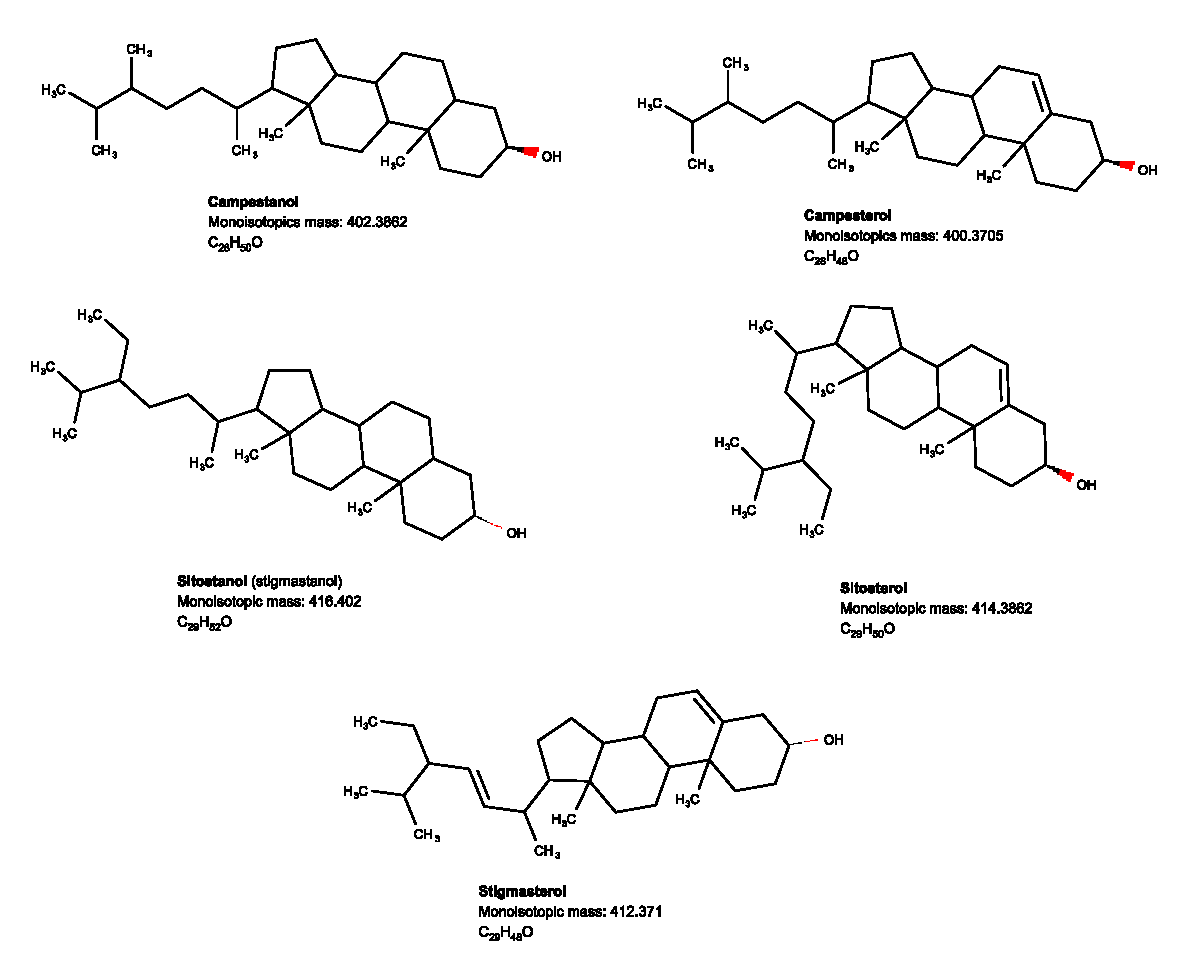
\includegraphics[scale=0.5]{images/5sterols_combined.eps}
    \caption{Major sterols in barley)}
    \label{fig:5sterol}
\end{figure}

Figure \ref{fig:5sterol} showed 5 major existed phytosterols in barley and were quantified\cite{sterol}. These 5 major types makes up around 90\% of total phytosterols\cite{sterol}. Still some minor sterols has not been identified yet.
We putatively identified the structure of this compound\ref{fig:putativesterol}. This proposal needs to be further validated.

\begin{figure}[H]
    \centering
    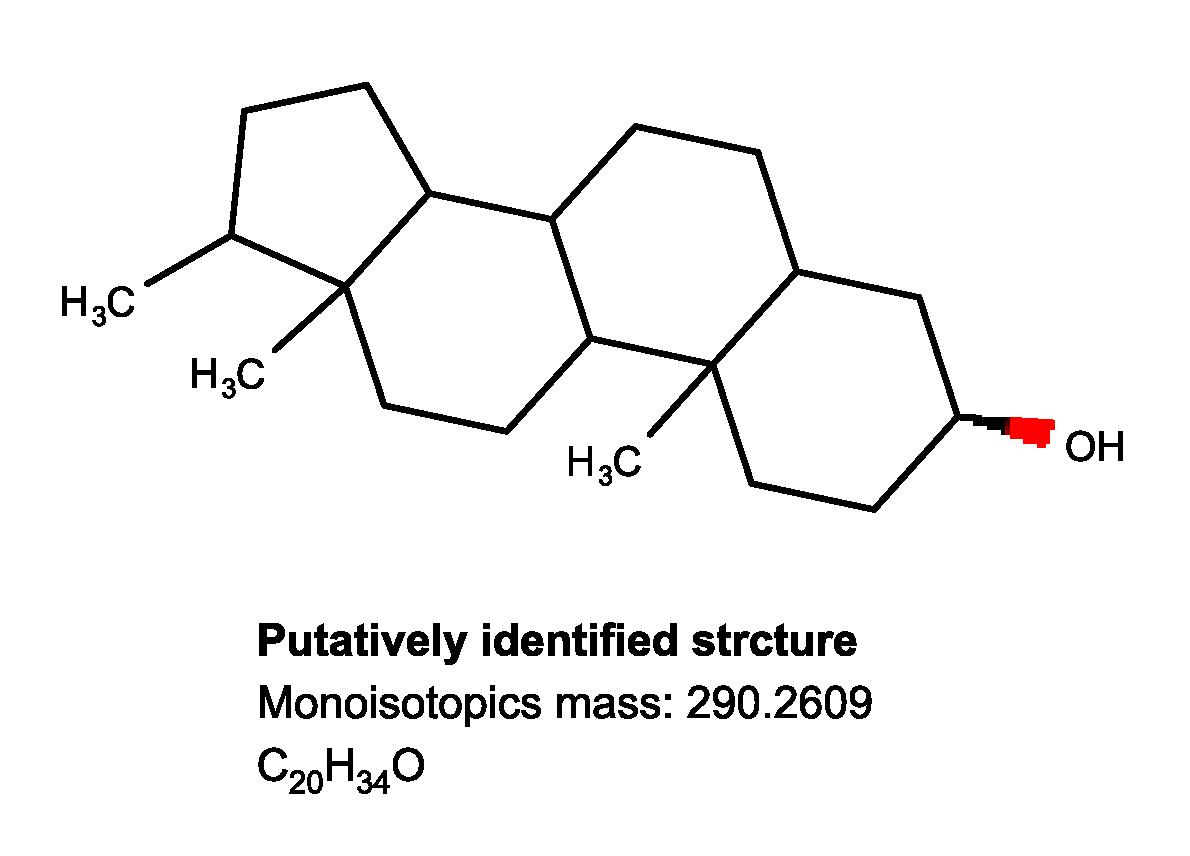
\includegraphics[scale=0.3]{images/possiblesterol.eps}
    \caption{Putatively identified structure}
    \label{fig:putativesterol}
\end{figure}